% !TEX root = scheduler.tex
\section{Design of the Scheduler}\label{sec:design}
In this section we present an overview of the components in the proposed \sys{} scheduler.
%, and its various components. the \textit{Policy Enforcer} and the \textit{Learning Agent}. 

\subsection{Scheduler Architecture Overview}\label{ssec:scheduler-arch}
Figure~\ref{fig:scheduler-architecture} shows the architecture of the \sys{} scheduler.
We first describe the \textit{Query Manager}. 
Each query in the system has its own instance of the Query Manager.
It manages the progress of the query that it owns.
The Query Manager maintains the query plan DAG and a data structure called
the \textit{Work Order Container} to track all the work orders that are ready for
scheduling. 
Recall from Section~\ref{sec:background}, a description of the work 
carried out on a block of data is a \textit{work order}. 

\begin{figure}
	\centering
	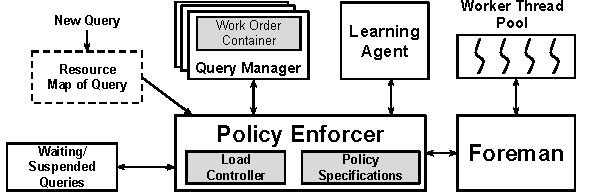
\includegraphics[width=\columnwidth]{figures/Scheduler-Architecture.pdf}
	\vspace*{-1.5em}
	\caption{Overview of the scheduler}
	\label{fig:scheduler-architecture}
	\vspace*{-1.5em}
\end{figure}

The Query Manager generates schedulable work orders for each active operator node
in the DAG. %, and stores them in the Work Order Container.
It also runs the core algorithm to determine when to activate nodes in the DAG. 
%Details about work orders are presented in Section~\ref{ssec:workorders}.
The Query Manager DAG node processing algorithm is a simple iterative DAG traversal algorithm, described in Appendix~\ref{apx:DAG-algo}. 

An important component of the system is the \textit{Policy Enforcer}. 
It selects a query among all the concurrent queries, and schedules its work order for execution. 
This in essence is a scheduling decision, and is taken based on a high-level policy provided to the system.
The policy is described in \textit{Policy Specifications}, which is an
abstraction that governs how resources are shared among concurrent queries. 

A two-way communication happens between the Policy Enforcer and the various Query Managers.
The Policy Enforcer requests a Query Manager to return a certain number of work orders from the query that it manages.
These work orders are then dispatched for execution by the Policy Enforcer. 
The Policy Enforcer communicates with the Query Manager upon every work order
completion, so that the Query Manager can then decide if new nodes in the DAG
can be activated, and if existing nodes can be marked as completed.
A detailed description of the Policy Enforcer is present in Section~\ref{ssec:policy-enforcer}. 

The Policy Enforcer contains a \textit{Load Controller} module, which is
responsible for ensuring that the system has enough resources to meet the
demands.
A new query in the system presents its resource requirements in the form of a
\textit{Resource Map} to the Load Controller.
The Resource Map describes the estimated resource requirements of the query
during its lifetime. 
An example Resource Map is shown below:%in Table~\ref{table:sample-resource-map}.
\begin{lstlisting}[language=python, 
								   basicstyle=\ttfamily\small, 
								   showstringspaces=false,
								   keywordstyle=\color{bondiblue}\bfseries, 
								   emph={CPU, Memory}, 
								   emphstyle=\color{cardinal}\bfseries]
CPU:    {min: 1 Core, max: 20 Cores}
Memory: {min: 20 MB,  max: 100 MB}
\end{lstlisting}
\vspace{-0.5em}
%\begin{table}[h]
%	\centering
%	\begin{tabular}{|p{0.2\columnwidth}|p{0.3\columnwidth}|p{0.3\columnwidth}|}
%		\hline
%		\textbf{Resource} & \textbf{Estimated min requirement} & \textbf{Estimated max requirement} \\ \hline
%		CPU & 1 Core & 20 Cores \\ \hline
%		Memory & 20 MB & 100 MB \\ \hline
%	\end{tabular}
%	\vspace{0.5em}
%	\caption{A sample resource map}
%	\label{table:sample-resource-map}
%	\vspace{-1.5em}
%\end{table}

This Resource Map states that the query can use 1 to 20 cores (i.e. specifies the range of intra-operator parallelism) and is estimated to require a minimum of 20 MB of memory to run, and an estimated 100 MB of memory in the worst case.
%The estimates provided in Resource Map can come from the query optimizer or some
%other mechanism, which is irrelevant to the scheduler.
The Load Controller determines the action to be taken with the new query. 
If enough resources are available, it admits the query.
If the system can potentially thrash due to the admission of the new query, it
can take a number of decisions, including wait-listing the query or
suspending one or more queries that are currently running to free up resources for the new query.
The Policy Enforcer maintains queues for wait-listed and suspended queries as shown in Figure~\ref{fig:scheduler-architecture}.
The Load Controller is described in detail in Section~\ref{ssec:load-control-mech}.

%A new query in the form of a DAG from the optimizer is sent to the Policy Enforcer.
%It decides when to activate or deactivate an entire query,
%as a means to \textit{admission control}. 
%The current admission control is simple and limits the number of concurrent 
%queries to a pre-defined number.  
%(It is easy to extend this component to examine factors such as buffer pool 
%swapping activity or cache miss rates to realize a different load control policy.)

The Policy Enforcer works with another module called the \textit{Learning Agent}. 
Execution statistics of completed work orders are passed from the Policy Enforcer to the Learning Agent.
This component uses a simple learning-based method to predict the time to 
complete future work orders using the execution times of finished work orders. 
Such predictions form the basis for the Policy Enforcer's decisions regarding scheduling the next set of work orders. 

%Work orders that are ready to execute are sent to a \textit{Foreman} module. 
%The Foreman simply acts as a link between the overall scheduler and a pool of 
%worker threads. 
The \textit{Foreman} module acts as a link between the Policy Enforcer and a pool of worker threads. 
It receives work orders that are ready for execution from the Policy Enforcer, and dispatches them to the worker threads. 
The Foreman can monitor the number of pending work orders for each worker, and 
use that information for load-balancing in work order dispatch.
When a worker completes executing a single work order, it sends a completion message 
to the Foreman.
This message contains statistics about the work order execution, which the Foreman passes on to the Policy Enforcer. 
During a work order execution, output data may be created (in blocks in the buffer pool). 
When an output data block is filled, the worker thread sends a message to the 
Foreman informing it about the filled block. 
The Foreman then forwards this information to the Policy Enforcer, 
which in turn communicates this information to the Query Manager. 
The Query Manager may then create a new work order based on this information;
e.g. if this block should be pipelined to another operator in the query plan.
%Next, we describe \sys{} schedulers's thread organization model. 

\sys{} has two kinds of threads - a scheduler thread and many worker threads that perform the actual relational operations as defined by \textit{work orders}. 
More details about the thread model are found in Appendix~\ref{apx:thread}

%\subsection{Work Orders}\label{ssec:workorders}
%Work done for executing a query in \sys{} is split into multiple \textit{work 
%orders}, as highlighted in Section~\ref{sec:background}. 
%A work order contains all the information that is needed to process tuples in a given 
%data block. 
%A work order encapsulates the relational operator that is being applied, the relevant 
%input relation(s), location of the input data block, any predicate(s) to be 
%applied on the tuples in the input block, and descriptors to other run-time 
%structures (such as hash tables).
%%The input data location is specified in terms of a unique storage block ID, a join hash table identifier, or an aggregation hash table identifier. 
%%In NUMA settings, a work order can also provide a preferred site for execution in the 
%%form of a NUMA socket ID. 
%%The scheduler then uses this information to make a 
%%\textit{data-locality aware} scheduling decision. \reminder{Should we remove NUMA 
%%because there are no experiments?}
%
%Consider the following full table scan query to illustrate the work order concept:

%\begin{lstlisting}[language=SQL, 
%basicstyle=\ttfamily\small, 
%showstringspaces=false,
%keywordstyle=\color{cardinal}\bfseries, 
%emph={San,Diego}, 
%emphstyle=\color{bondiblue}\bfseries]
%SELECT name FROM Employee WHERE city=`San Diego'
%\end{lstlisting}	
%\vspace{-0.4em}

%The plan for this query has a simple \textit{selection} operator.  
%For the selection operator, the number of work orders is same as the number of input blocks in the \verb+Employee+ table. 
%Each selection work order contains the following information:
%\begin{itemize}
%\itemsep0.1em
%\item {Relation: \verb+Employee+, attribute: \verb|name|}
%\item {Predicate: \lstinline[language=SQL, 
%                                   basicstyle=\ttfamily\small, 
%                                   keywordstyle=\color{cardinal} \bfseries,
%                                   emph={San,Diego}, 
%                                   emphstyle=\color{bondiblue}\bfseries]|city=`San Diego'|}
%\item {The unique ID of an input block from the \verb+Employee+ table}
%\end{itemize}
%
%The work orders for a join operation %(illustrated below) 
%are slightly more complicated. 
%For example, a \textit{probe work order},  contains the unique ID of the probe 
%block, 
%%(as described in Section~\ref{ssec:storage-manager}, a hash table is stored in a block in the buffer pool), build and probe relations, 
%a pointer to the hash table, the projected attributes, and the join predicate.
%%Each operator algorithm (e.g. a scan or the build/probe phase of a hash-join) 
%%in the system has a C++ class that is derived from 
%%a root abstract base class that has a virtual method called \verb|execute()|.
%%Executing a work order simply involves calling the \verb|execute()| method 
%%on the appropriate operator algorithm C++ class object. 

\begin{figure}[h]
	\centering
	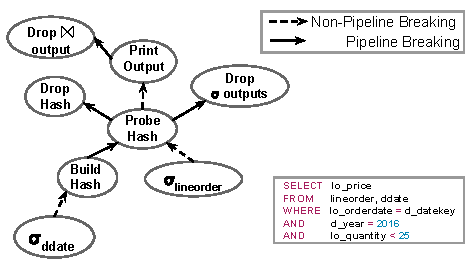
\includegraphics[width=\columnwidth]{figures/QueryPlan.pdf}
	\vspace*{-2em}
	\caption{A join query and its DAG}
	\label{fig:dag}
%	\vspace*{-1.5em}
\end{figure}

\subsection{Policy Enforcer}\label{ssec:policy-enforcer}
The Policy Enforcer assigns a probability value to each active query in the system. 
The scheduling decisions are taken based on these probabilities. 
\reminder{Update the line below}
We also saw the connection between the probability value and the execution time of future work order, with fair policy as a case in point. 
We describe the Policy Enforcer in depth in Appendix~\ref{apx:policy-enforcer}.

However this raises some questions: How do we know the future execution time of a work order? 
%Second, what happens if the future execution time of work orders keep changing? 
Why should we compute the probability using future work order execution times instead of assigning fixed probabilities to queries?
We answer these questions by introducing a Learning agent module in the next section. 
 
%In the beginning of a workload execution, the Policy Enforcer uses some default 
%probability values until the Learning Agent collects enough data so as to make a prediction. 
\subsection{Learning Agent}\label{ssec:learning}
The Learning Agent module is responsible for predicting the execution times of the future work orders for a given query. 
It gathers the history of executed work orders of a query and applies a prediction model on such a history to estimate the execution time of a future work order.
This predicted execution time is used to compute the probability assigned to each query (cf. Section~\ref{sec:policy} for probability derivations).  
%The Learning agent also helps us relax our earlier assumption, about knowledge of execution times of the future work orders for the queries. 
%In a real implementation, such information is not available.
%To get around this issue, we incorporate a Learning Agent module, described in the next section. 
%It predicts the execution time of future work orders, using a learning methodology. 
%Such predicted execution times are used to compute the probabilities assigned to the queries.

%In this section we describe the Learning Agent module in the scheduler. 
%As described in Section~\ref{ssec:policy-enforcer}, the Learning Agent converts predicted execution times of future work orders to probabilities, which are used for the scheduling decisions.
One might question the need of the Learning Agent and instead consider assigning a fixed probability value to each query (say $1/N$, with $N$ queries in the fair policy).
In the following section, we address this issue. 
A motivational example for the learning agent is described in Appendix~\ref{apx:learning-motivation}.
%Later we explain the methodology used by the Learning Agent.

It is clear that the work order execution times for both queries are different, and the difference between them changes over time. 
If the scheduler assigns the same probability to both queries (i.e. 0.5), it is equally likely to schedule a work order from either of them. 
As a result, the queries will have different CPU utilization times in a given epoch, thus resulting in an unfair CPU allocation. 
In order to be consistently fair in allocating CPU resources to the queries, we should continuously observe the work order execution times of queries and adjust the CPU allocation accordingly. % update the predicted work order execution times. 
%Later, we substantiate this explanation by an experiment (c.f. Section~\ref{ssec:learning-impact}).

In general, the time per work order metric doesn't stay the same throughout a query's lifetime.
In each phase of the query, the time per work order is different.
As the query plan gets bigger, the number of phases in the plan increase.
In addition, different queries may be in different phases at a given point in time.
To make things more complicated, queries can enter or leave the system at any time.

%$Q4.1$, the execution exhibits different ``phases'', each belonging to different relational operators in the query such as selection, building the hash table, probing the hash table, aggregation etc. 
%\reminder{Describe in the figure the begin and end times of various phases}

Therefore it is difficult to statically pick a proportion of CPU to allocate to the concurrent queries. 
Hence there is a need to ``learn'' the various phases in the query execution and dynamically change the proportion of resources allocated to each query, based on each query's phase.
Next, we study the methodology used by the Learning Agent.
\subsubsection{Learning Agent Methodology}
%The Learning Agent builds each query's \textit{execution profile} based 
%on the execution statistics of recently completed work orders for that query.
The Learning agent uses the execution times of previously executed work orders 
denoted as $t_{w_{1}}, t_{w_{2}}, \ldots, t_{w_{k}}$ to predict the execution time of 
the next work order $t_{w_{k+1}}$ for a given query.\footnote{In the beginning of a query execution, when enough information about work order execution times is not available, we use the default probabilities in the Policy Enforcer, instead of using default predicted times in the Learning Agent.}
Figure~\ref{fig:scheduler-cycle} shows the Learning Agent's interaction with the other scheduler components.
%It receives the execution statistics of an  executed work order, and uses this information 
%to predict the execution time of the future work orders. 

\begin{figure}[h]
	\centering
	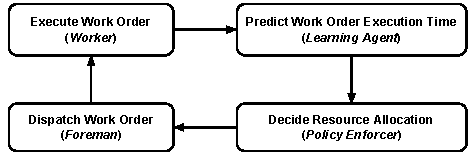
\includegraphics[width=\linewidth]{figures/Compact-SchedulerCycle.pdf}
	\vspace{-2em}
	\caption{Interactions among scheduler components}
	\label{fig:scheduler-cycle}
%	\vspace{-1.5em}
\end{figure}

The set of previously executed work orders can belong to multiple relational operators in the query operator DAG. 
The Learning Agent stores the execution times of the work orders grouped by their source relational operator, e.g. the execution statistics of select work orders are maintained together and kept separate from aggregation work orders. 

%A prediction model is used to estimate the execution time of future work orders. 
\sys{}'s scheduler currently uses linear regression as the prediction model.
We chose linear regression as it is fast, accurate, and efficient w.r.t. the computational and the memory storage overheads of the model. 
%(New models can be easily added using an abstraction mechanism.) 
To lower the CPU and memory overhead of the model, we limit the amount of execution statistics stored in the Learning Agent.
We discard records beyond a certain time window. 
When all the work orders of an operator finish execution, we remove its records completely. 
In a query, when multiple relational operators are active, 
linear regression combines the statistics of all active operators and predicts a single 
value for the next work order execution time.
%There are few reasons for the choice of our prediction methodology: We want a fast 
%technique so that the prediction itself doesn't become a  bottleneck in the core 
%execution 
%of the queries. The prediction method should be simple and reasonably accurate. The 
%linear regression approach is inexpensive and straightforward to reason about. It reacts 
%quickly and adapts well to the change of operators (and corresponding change in 
%execution times of work orders) that happen during the DAG traversal described in 
%Algorithm~\ref{alg:dag-traversal}.

We note that the problem of estimating the query execution time is well-studied 
~\cite{duggan2011performance, wu2013towards, li2012gslpi, 
chaudhuri2004estimating}. 
The Learning Agent does not require such methods. 
However, it can combine estimates from other methods with its simple learning-based estimates.
%i.e. we try to predict the execution times of immediate work orders, as opposed  to a 
%global
%level estimation that may involve estimation of the progress of the query and prediction
%of query/workload completion times. The Learning Agent can be extended to use
%other techniques for the prediction, and is complimentary to other methods for
%estimation.